\chapter{Redes de longa distância}\label{chp:roteamento}
%%% https://www.dailymotion.com/video/x11vklx
%%% https://www.youtube.com/watch?v=YdM7yBrtAck
Neste capítulo, vamos ligar duas redes locais para formar uma rede de longa distância (\textit{Wide Area Network} -- WAN). Para isso, as redes locais, que já estão interconectadas com \textit{switches}, vão utilizar os roteadores para se interconectar. Utilizaremos como base a estrutura ilustrada na \Cref{fig:roteamentoInicio} a seguir.

\begin{figure}[!hbt]
    \centering
    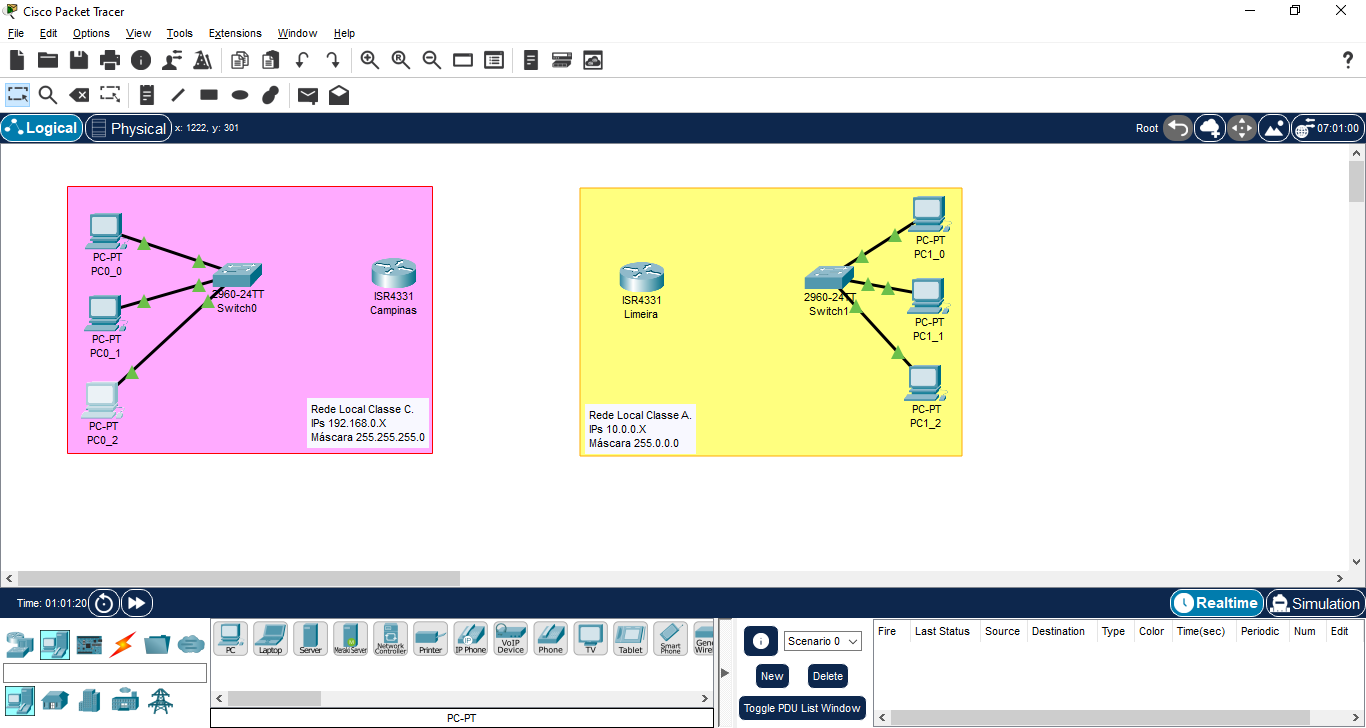
\includegraphics[width=.99\textwidth]{Figuras/InterRedesLocais}
    \caption{Redes locais que serão interligadas.}\label{fig:roteamentoInicio}
\end{figure}

De início, as redes locais da esquerda e da direita, ilustrada na \Cref{fig:roteamentoInicio}, são compostas, cada uma, por três PCs interligados a um \textit{switch} (Modelo 2960) com cabos par-trançados. Posteriormente, adicionaremos um roteador (modelo ISR 4331) em cada uma das redes e os interligaremos. Estamos supondo que a rede da esquerda está fisicamente em Campinas e a rede da direita está fisicamente em Limeira.

A rede da esquerda é uma rede local classe C. Portanto, os endereços IP estáticos são \texttt{192.168.0.X}, onde \texttt{X} é substituído por \texttt{2} no \texttt{PC0\_0}, \texttt{3} no \texttt{PC0\_1} e \texttt{4} no \texttt{PC0\_2}. A máscara em todos os PCs dessa rede é \texttt{255.255.255.0}. 

De forma análoga, a  rede da direita é uma rede local classe A. Portanto, os endereços IP estáticos são \texttt{10.0.0.X}, onde \texttt{X} é substituído por \texttt{2} no \texttt{PC1\_0}, \texttt{3} no \texttt{PC1\_1} e \texttt{4} no \texttt{PC1\_2}. A máscara em todos os PCs dessa rede é \texttt{255.0.0.0}. 

Certifique-se que as redes locais estejam funcionando normalmente antes de proceder com os próximos passos.

\section{Conexão da rede local a um roteador}\label{sec:conexaoRedeLocalRoteador}
Em cada uma das redes locais, vamos adicionar um roteador (modelo ISR 4331) e, posteriormente, ligá-lo a sua rede local com um cabo par trançado. A ligação será feita usando a porta \texttt{Gi\-ga\-bit\-Ether\-net\-0/1} do \textit{switch} à porta \texttt{Gi\-ga\-bit\-Ether\-net\-0/0/0} do roteador. O mesmo procedimento deverá ser feito para cada rede local. Para diferenciar os roteadores de cada rede local, vamos nomeá-los de \texttt{Campinas} e \texttt{Limeira}, respectivamente. 

Note que a conexão física está estabelecida, mas ainda não há transmissão de dados entre os roteadores. Então, precisamos configurá-los.

\subsection{Configuração dos roteadores para conexão com a LAN}\label{subsec:configRoreadores}
Para configurar cada um dos roteadores, precisamos acessar a interface da linha de comando (CLI). Para isso, clique em um dos roteadores e, depois, selecione a aba \texttt{CLI}.

Uma janela aparecerá, perguntando se você quer entrar na configuração do roteador (\textit{Would you like to enter basic management setup? [yes/no]}). Digite \semaspas{no} e pressione \keys{\enter}. O \textit{prompt} com a \textit{string} \enquote{\texttt{Router>}} mostrará que está pronto para receber os comandos. Agora execute os passos a seguir.

\begin{enumerate}[label*=\arabic*.]
    \item Digite \semaspas{enable} para entrar no modo administrador. Note que o \textit{prompt} mudou para \enquote{\texttt{Router\#}}.
    \item Digite \semaspas{conf terminal} para entrar na configuração global. Note que o \textit{prompt} mudou para \enquote{\texttt{Router (config)\#}}.
    \item Agora defina o nome do roteador. Para isso, digite \semaspas{hostname Campinas} para definir o nome desse roteador. Note que para o outro roteador, você deverá atribuir outro nome (\texttt{Limeira}).
    \item Verifique se as configurações até o momento estão de acordo. Para isso execute os seguintes passos:
    \begin{enumerate}[label*=\arabic*.]
        \item Digite \semaspas{exit} para sair do modo configuração.
        \item Digite \semaspas{show running-config} para mostrar a configuração até o momento.
    \end{enumerate}
\end{enumerate}

Note que o \texttt{hostname} está configurado, mas as interfaces \textit{GigabitEthernet} não têm endereços IP atribuído a elas e também estão desligadas (\texttt{shutdown}). Vamos então, configurar a conexão entre o roteador (\texttt{Campinas}) à sua rede local. Para tanto, execute  os próximos passos ainda na CLI.

\begin{enumerate}[label*=\arabic*.]
    \item Digite novamente \semaspas{conf terminal} para entrar na configuração global. 
    \item Digite \semaspas{interface GigabitEthernet 0/0/0} para configurar a interface à qual o \textit{switch} está conectado.
    \item Atribua o IP e a máscara à essa interface com o comando a seguir:
    
       \texttt{\textcolor{green}{Campinas(config-if)\#} \textcolor{blue}{ip} address 192.168.0.1 255.255.255.0}

    \item Em seguida, ligue a porta e a mantenha ligada com o comando \semaspas{no shutdown}.
    \item Por uma questão de organização, vamos atribuir uma descrição para essa interface com o comando \Comando{description}. Note que, após o comando, vem a descrição daquela interface. Usaremos o comando a seguir:
    
       \texttt{\textcolor{green}{Campinas(config-if)\#} \textcolor{blue}{description} Porta LAN Campinas}
       
    \item Verifique se as configurações até o momento estão de acordo. Para isso execute os seguintes passos:
    \begin{enumerate}[label*=\arabic*.]
        \item Digite \semaspas{exit}  duas vezes para sair do modo de configuração da interface e do modo de configuração global.
        \item Digite \semaspas{show running-config} para mostrar a configuração até o momento.
    \end{enumerate}
\end{enumerate}

Repita o mesmo procedimento para o roteador em Limeira. Note que o endereço IP do roteador será \texttt{10.0.0.1} e a máscara \texttt{255.0.0.0}.

\section{Conexão dos roteadores entre si}\label{subsec:conexaoRoteadores}
Depois que cada rede local está conectada ao seu respectivo roteador, vamos conectar os roteadores entre si. Nós utilizaremos um cabo par trançado e conectaremos ambos os roteadores nas respectivas portas \texttt{Gi\-ga\-bit\-Ether\-net\-0/0/1}.

É importante lembrar que teremos, conceitualmente, três redes: LAN de Campinas (\texttt{192.168.0.0}), a LAN de Limeira (\texttt{10.0.0.0}) e a WAN que interliga ambas as redes (\texttt{200.100.10.0}). Para a WAN, definimos que os roteadores terão os IPs \texttt{200.100.10.1} para Campinas e \texttt{200.100.10.2} para Limeira, ambas com a máscara \texttt{255.255.255.0}. 

Para a configuração dos roteadores, será preciso executar os passos a seguir. Faremos inicialmente no roteador que está em \texttt{Campinas}.
\begin{enumerate}[label*=\arabic*.]
  \item Entre novamente na interface da linha de comando do roteador (veja detalhes no início da \Cref{subsec:configRoreadores}).
  \item Digite \semaspas{enable} para entrar no modo administrador. 
  \item Digite \semaspas{conf terminal} para entrar na configuração global.
  \item Defina a interface que será configurada. Nesse caso, vamos usar a interface que liga este roteador ao roteador de \texttt{Limeira}. Use o comando a seguir:

    \texttt{\textcolor{green}{Campinas(config)\#} \textcolor{blue}{interface} GigabitEthernet0/0/1}
  
  \item Atribua o IP e a máscara à essa interface e informe que a interface estará ativa com os comandos a seguir. Note que geralmente esses IP e máscara são atribuídos por uma empresa de telecomunicações, responsável pela rede de longa distância. Nesse exemplo, usaremos o IP \texttt{200.100.10.1} com a máscara \texttt{255.255.255.0}.
    
       \texttt{\textcolor{green}{Campinas(config-if)\#} \textcolor{blue}{ip} address 200.100.10.1 255.255.255.0}

       \texttt{\textcolor{green}{Campinas(config-if)\#} \textcolor{blue}{no shutdown}}

   \item Por uma questão de organização, vamos atribuir uma descrição para essa interface com o comando \Comando{description}. Note que, após o comando, vem a descrição daquela interface. Usaremos o comando a seguir:
    
       \texttt{\textcolor{green}{Campinas(config-if)\#} \textcolor{blue}{description} Porta WAN Campinas-Limeira}

   \item Para uma configuração mais precisa, vamos usar o comando \Comando{bandwidth} para estabelecer a largura de banda dessa conexão. Como é uma \textit{Gigabit Ethernet}, vamos estabelecer uma largura de banda de 125.000.000 \textit{bytes} por segundo (Bps). Para isso, usamos o comando a seguir. Perceba que o valor está em \textit{kilobytes}. Portanto, 125.000.000 bytes por segundo é 125000 \textit{kilobytes} por segundo (KBps).
   
       \texttt{\textcolor{green}{Campinas(config-if)\#} \textcolor{blue}{bandwidth} 125000}

  \item Saia da configuração da interface com o comando \semaspas{exit} e vamos configurar o protocolo de roteamento \textit{Routing Information Protocol} (RIP) com o comando a seguir. Note que poderíamos usar outros protocolos como o \textit{Border Gateway Protocol} (BGP), \textit{Enhanced Interior Gateway Routing Protocol} (EIGRP) ou \textit{Open Shortest Path First} (OSPF).

        \texttt{\textcolor{green}{Campinas(config)\#} \textcolor{blue}{router} rip}
  
  \begin{enumerate}[label*=\arabic*.]
    \item Note que o \textit{prompt} mudou para \enquote{\texttt{Campinas(config-router)\#}}. Agora, vamos informar as três redes às quais o roteador está conectado com os comandos a seguir. 

        \texttt{\textcolor{green}{Campinas(config-router)\#} \textcolor{blue}{network} 192.168.0.0}

        \texttt{\textcolor{green}{Campinas(config-router)\#} \textcolor{blue}{network} 10.0.0.0}

        \texttt{\textcolor{green}{Campinas(config-router)\#} \textcolor{blue}{network} 200.100.10.0}

    \item Volte à configuração do terminal digitando o comando \Comando{exit} e pressionando a tecla \keys{\enter} \underline{duas vezes}. Eventualmente, você poderá digitar \semaspas{end} ou simplesmente pressionar \keys{\ctrl + Z}.
  \end{enumerate}
  
  \item Note que todas essas configurações estão na memória, mas não foram salvas. Para salvá-las de forma permanente, use o comando a seguir e pressione \keys{\enter} em seguida:

       \texttt{\textcolor{green}{Campinas\#} \textcolor{blue}{copy} running-config startup-config}
  \begin{enumerate}[label*=\arabic*.]
    \item Confirme que a configuração foi salva usando o comando a seguir:

      \texttt{\textcolor{green}{Campinas\#} \textcolor{blue}{show} startup-config}
  \end{enumerate}
\end{enumerate}

Agora, basta repetir o mesmo procedimento para o roteador em \texttt{Limeira}. Não esqueça de substituir os endereços e máscaras das respectivas redes. A lista de comandos a serem executados no roteador de Limeira é a seguinte:
\begin{itemize}
    \item \texttt{\textcolor{green}{Campinas(config-if)\#} \textcolor{blue}{interface} GigabitEthernet0/0/1}
    \item \texttt{\textcolor{green}{Router>} \textcolor{blue}{enable}}
\item \texttt{\textcolor{green}{Router\#} \textcolor{blue}{conf} terminal}
\item \texttt{\textcolor{green}{Router(config)\#} \textcolor{blue}{hostname} Limeira}
\item \texttt{\textcolor{green}{Limeira(config)\#} \textcolor{blue}{interface} GigabitEthernet 0/0/0}
\item \texttt{\textcolor{green}{Limeira(config-if)\#} \textcolor{blue}{ip} address 10.0.0.1 255.0.0.0}
\item \texttt{\textcolor{green}{Limeira(config-if)\#} \textcolor{blue}{no} shutdown}
\item \texttt{\textcolor{green}{Limeira(config-if)\#} \textcolor{blue}{description} Porta LAN Limeira}
\item \texttt{\textcolor{green}{Limeira(config-if)\#} \textcolor{blue}{exit}}
\item \texttt{\textcolor{green}{Limeira(config)\#} \textcolor{blue}{interface} GigabitEthernet0/0/1}
\item \texttt{\textcolor{green}{Limeira(config-if)\#} \textcolor{blue}{ip} address 200.100.10.2 255.255.255.0}
\item \texttt{\textcolor{green}{Limeira(config-if)\#} \textcolor{blue}{no} shutdown}
\item \texttt{\textcolor{green}{Limeira(config-if)\#} \textcolor{blue}{description} Porta WAN Limeira-Campinas}
\item \texttt{\textcolor{green}{Limeira(config-if)\#} \textcolor{blue}{bandwidth} 125000}
\item \texttt{\textcolor{green}{Limeira(config-if)\#} \textcolor{blue}{exit}}
\item \texttt{\textcolor{green}{Limeira(config)\#} \textcolor{blue}{router} rip}
\item \texttt{\textcolor{green}{Limeira(config-router)\#} \textcolor{blue}{network} 192.168.0.0}
\item \texttt{\textcolor{green}{Limeira(config-router)\#} \textcolor{blue}{network} 10.0.0.0}
\item \texttt{\textcolor{green}{Limeira(config-router)\#} \textcolor{blue}{network} 200.100.10.0}
\item \texttt{\textcolor{green}{Limeira(config-router)\#} \textcolor{blue}{exit}}
\item \texttt{\textcolor{green}{Limeira\#} \textcolor{blue}{exit}}
\item \texttt{\textcolor{green}{Limeira\#} \textcolor{blue}{copy} running-config startup-config}
\end{itemize}

Confirme que todos os computadores estão de fato conectados, executando o \Comando{ping} de um computador na rede de Limeira, para o IP de um computador que está na rede de Campinas.

\section{Exercício}
Adicione a rede atual mais uma rede Local em Piracicaba. Em seguida, adicione um roteador à rede de Piracicaba e interligue-o aos demais roteadores. Faça as devidas configurações e teste para ver se todas as redes estão alcançáveis entre si.

\section{Configuração de roteadores com DHCP}
Ao configurar as redes de longa distância anteriores, nós definimos um endereço IP fixo para todos os computadores. No entanto, a utilização do DHCP permitirá a adição de novos computadores à rede local, sem que seja necessário se preocupar com a configuração manual dos endereços IP.

Para isso, escolha um dos roteadores (nesse exemplo, escolheremos o roteador de Limeira), clique sobre ele e entre na CLI. Depois, execute os passos a seguir:

\begin{enumerate}[label*=\arabic*.]
   \item Digite \semaspas{enable} para entrar no modo administrador.
   \item Digite \semaspas{conf terminal} para entrar na configuração global.
   \item Crie e nomeie um \textit{pool} (agrupamento) de endereços IP que serão atribuídos pelo DHCP com o comando a seguir. Nesse caso, o nome que utilizaremos será \texttt{dhcpLimeira}.

    \texttt{\textcolor{green}{Limeira(config)\#} \textcolor{blue}{ip} ip dhcp pool dhcpLimeira}

   \item Para garantir, vamos definir a rede padrão com os comandos a seguir: 
   
     \texttt{\textcolor{green}{Limeira(dhcp-config)\#} \textcolor{blue}{network} 10.0.0.0 255.0.0.0}
     
     \texttt{\textcolor{green}{Limeira(dhcp-config)\#} \textcolor{blue}{default-router} 10.0.0.1}

    \item Agora, vamos excluir uma faixa de endereços IP do \textit{pool}, que vai de \texttt{10.0.0.1} a \texttt{10.0.0.9}. Isso é necessário para garantir que o roteador e alguns outros endereços IPs não sejam atribuídos pelo DHCP. Com isso, evitamos colisões do roteador com outros IPs. Usaremos o comando a seguir:
     
     \texttt{\textcolor{green}{Limeira(dhcp-config)\#} \textcolor{blue}{ip} dhcp excluded-address 10.0.0.1 10.0.0.9}

     \item Terminada a configuração, é preciso sair com o \Comando{exit} e depois salvar as configurações. Use o comando a seguir para salvá-las.

       \texttt{\textcolor{green}{Limeira\#} \textcolor{blue}{copy} running-config startup-config}
\end{enumerate}

Não esqueça de alterar as configurações de cada PC da LAN de Limeira para utilizar o DHCP ao invés de endereços IP estáticos. Para isso, para cada PC, faça o seguinte: Clique sobre o PC, depois clique na aba \texttt{Desktop} e, em seguida, em \texttt{IP Configuration}. Na Seção \texttt{IP Configuration} selecione a opção DHCP.

\section{Exercício}
Altere as demais LANs para usarem DHCP.